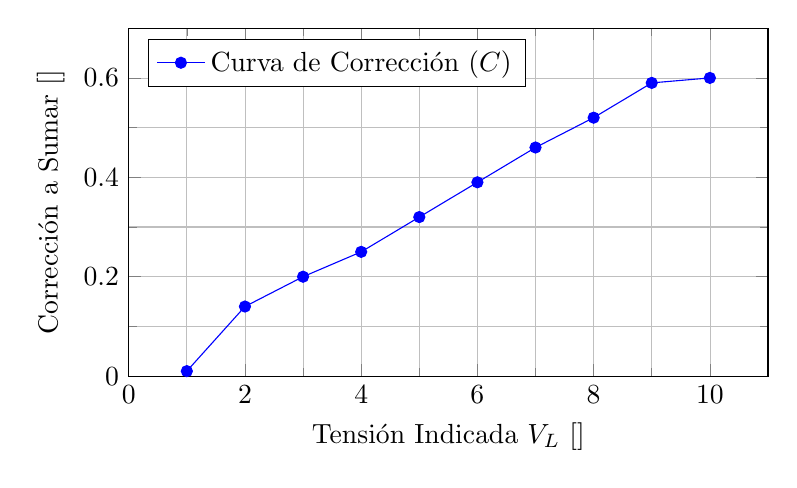
\begin{tikzpicture}
    \begin{axis}[
        width=0.8\textwidth,
        height=6cm,
        xlabel={Tensión Indicada $V_L$ [$\V$]},
        ylabel={Corrección a Sumar [$\V$]},
        xmin=0, xmax=11,
        ymin=0, ymax=0.7,
        grid=both,
        minor tick num=1,
        major grid style={line width=.2pt,draw=gray!50},
        legend pos=north west
    ]
    \addplot[color=blue, mark=*] coordinates {
        (1, 0.01)
        (2, 0.14)
        (3, 0.20)
        (4, 0.25)
        (5, 0.32)
        (6, 0.39)
        (7, 0.46)
        (8, 0.52)
        (9, 0.59)
        (10, 0.60)
    };
    \legend{Curva de Corrección ($C$)}
    \end{axis}
\end{tikzpicture}
